Laser Harp consists of four layers. The first layer is the power system, which is going to act as a power source for the device and consists of battery or similar power source. Second layer is frames and components which consists of laser beams, receptors, mister and speaker. Receptors are going to identify the interference in the laser beam and send the signal towards MIDI converter. Mister is being used for visibility whereas speakers are for audio output. Then, we have MIDI converter which is going to receive signals from the receptors and encode those signals as MIDI signals. Finally, the last layer is the sound module which is going to decode the MIDI signals, pass the resulting outcome to fluid synth which inturn sends the audio signals to speakers via soundcard. 

\begin{figure}[h!]
	\centering
 	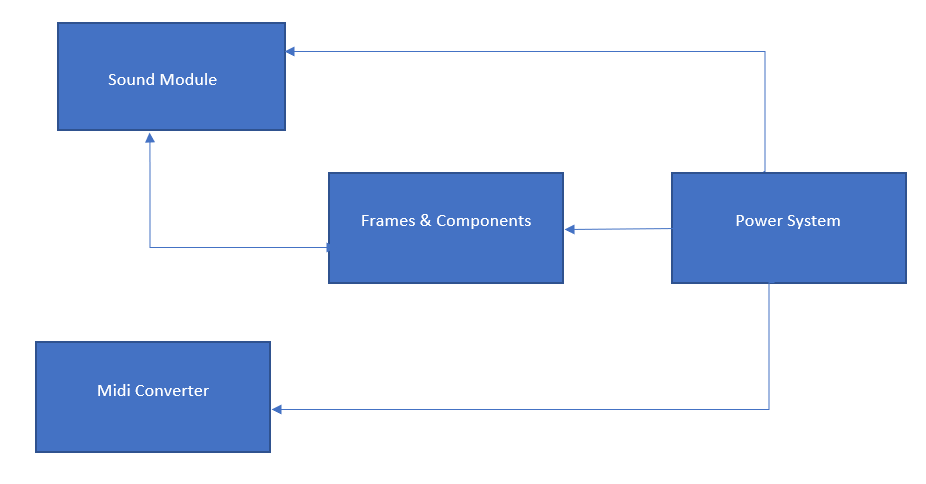
\includegraphics[width=0.60\textwidth]{images/layers}
 \caption{Laser Harp Architectural Layer Diagram}
\end{figure}

\subsection{Layer X Description}
Each layer should be described separately in detail. Descriptions should include the features, functions, critical interfaces and interactions of the layer. The description should clearly define the services that the layer provides. Also include any conventions that your team will use in describing the structure: naming conventions for layers, subsystems, modules, and data flows; interface specifications; how layers and subsystems are defined; etc. 

\subsection{Layer Y Description}
Each layer should be described separately in detail. Descriptions should include the features, functions, critical interfaces and interactions of the layer. The description should clearly define the services that the layer provides. Also include any conventions that your team will use in describing the structure: naming conventions for layers, subsystems, modules, and data flows; interface specifications; how layers and subsystems are defined; etc. 

\subsection{Layer Z Description}
Each layer should be described separately in detail. Descriptions should include the features, functions, critical interfaces and interactions of the layer. The description should clearly define the services that the layer provides. Also include any conventions that your team will use in describing the structure: naming conventions for layers, subsystems, modules, and data flows; interface specifications; how layers and subsystems are defined; etc. 
